
\chapter{Introduzione ai grafi}

\section{Grafo}

\begin{center}
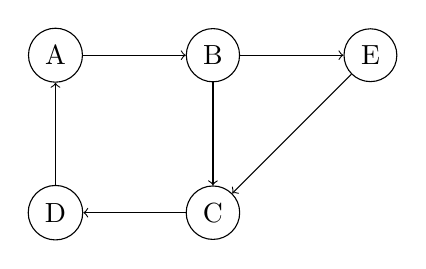
\begin{tikzpicture}
  % Nodi
  \node[draw, circle] (A) at (0,0) {A};
  \node[draw, circle] (B) at (2,0) {B};
  \node[draw, circle] (C) at (2,-2) {C};
  \node[draw, circle] (D) at (0,-2) {D};
  \node[draw, circle] (E) at (4,0) {E};

  % Archi
  \draw[->] (A) -- (B);
  \draw[->] (B) -- (C);
  \draw[->] (C) -- (D);
  \draw[->] (D) -- (A);
  \draw[->] (B) -- (E);
  \draw[->] (E) -- (C);
\end{tikzpicture}
\end{center}

Un grafo $G$ \`e costruti da una coppia di insieme $(V, A)$, dove $V$ \`e l'insieme dei vertici e $A$ \`e l'insieme degli archi.


Esistono due tipi di grafi:
\begin{itemize}
  \item \textbf{Grafo orientato}: gli archi sono orientati, ovvero $(u,v) \neq (v,u)$.
  \item \textbf{Grafo non orientato}: gli archi non sono orientati, ovvero $(u,v) = (v,u)$.
\end{itemize}



\subsection{Liste di adiacenza}
Per rappresentare un grafo si possono utilizzare le liste di adiacenza, un esempio \`e il seguente:

\begin{center}
\begin{tabular}{l|l}
Nodo & Adiacenti \\
\hline
A & B, D \\
B & A, C \\
C & B, D \\
D & A, C \\
\end{tabular}
\end{center}


\subsection{Matrice di adiacenza}

Se il grafo \`e \textbf{orientato} la matrice di adiacenza \`e la seguente:

\begin{center}
  \[
\begin{array}{c|cccc}
  & A & B & C & D \\
\hline
A & 0 & 1 & 0 & 1 \\
B & 0 & 0 & 1 & 0 \\
C & 0 & 0 & 0 & 1 \\
D & 1 & 0 & 0 & 0 \\
\end{array}
\]
\end{center}
Le righe rappresentano i nodi di partenza degli archi, mentre le colonne rappresentano i nodi di arrivo. Gli elementi della matrice indicano se c'è un arco che collega i nodi (1 se c'è un arco, 0 altrimenti).



Se il grafo \`e \textbf{non orientato} la matrice di adiacenza \`e la seguente:

\begin{center}
  \[
\begin{array}{c|cccc}
  & A & B & C & D \\
\hline
A & 0 & 1 & 0 & 1 \\
B & 1 & 0 & 1 & 0 \\
C & 0 & 1 & 0 & 1 \\
D & 1 & 0 & 1 & 0 \\
\end{array}
\]
\end{center}
 Le righe e le colonne rappresentano i nodi del grafo, mentre gli elementi della matrice indicano se due nodi sono adiacenti (1 se sono adiacenti, 0 altrimenti).


 \subsection{Cammino}
 Un cammino \`e una sequenza di vertici e di archi che collegano due vertici.
 Esistono diverse tipologie di cammini:
 \begin{itemize}
   \item \textbf{Cammino semplice}: un cammino in cui non ci sono archi percosi pi\`u di una volta.
   \item \textbf{Cammino elementare}: un cammino in cui non un nodo non \`e percorso pi\`u di una volta.
 \end{itemize}

 \subsection{Ciclo}
  Un ciclo \`e un cammino in cui il nodo di partenza \`e uguale al nodo di arrivo.
  

  \subsection{Circuiti Hamiltoniani}

  Un circuito Hamiltoniano \`e un ciclo che passa per tutti i nodi del grafo una e una sola volta.


  \subsection{Componenti connesse}
  Dati due nodi $u$ e $v$ di un grafo $G$, si dice che $u$ e $v$ sono connessi se esiste un cammino che collega $u$ e $v$.



  \subsection{Grafo completo}
  Un grafo \`e completo se ogni coppia di nodi \`e collegata da un arco.

  % \subsection{Sottografo e grafo partiale}
  % Dato un grafo $G = (V, A)$, un sottografo $G' = (V', A')$ \`e un grafo tale che $V' \subseteq V$ e $A' \subseteq A$.


  \subsection{Matching}
  Un matching \`e un sottoinsieme di archi di un grafo tale che ogni nodo \`e collegato ad al massimo un arco del matching.


  \subsection{Grafo bipartito}
  Un grafo \`e bipartito se i suoi nodi possono essere divisi in due insiemi $V_1$ e $V_2$ tali che ogni arco del grafo collega un nodo di $V_1$ con un nodo di $V_2$.




  \subsection{Albero}
  Un albero \`e un grafo connesso e aciclico.

  \subsubsection{Albero di supporto}
  Un albero di supporto di un grafo $G$ \`e un sottografo di $G$ che \`e un albero e che contiene tutti i nodi di $G$.
